\documentclass[12pt,letterpaper]{article}
\usepackage{graphicx}
\usepackage[utf8]{inputenc}
\usepackage{mathtools}
\usepackage[margin=0.5in]{geometry}
\usepackage{booktabs}
\usepackage{tabu}
\usepackage{caption}
\usepackage{wasysym}
\usepackage{siunitx}
\usepackage[labelfont=bf, skip=5pt, font=small]{caption}
\usepackage{hyperref}
\hypersetup{
    colorlinks=true,
    linkcolor=blue,
    filecolor=magenta,      
    urlcolor=cyan,
    pdftitle={Overleaf Example},
    pdfpagemode=FullScreen,
    }
\usepackage[font=footnotesize,labelfont=bf]{caption}
\setlength{\parskip}{1em}
\setlength{\parindent}{0em}


\let\DeclareUSUnit\DeclareSIUnit
\let\US\SI
\DeclareUSUnit\inch{in}
\DeclareUSUnit\lbf{lbf}
\DeclareUSUnit\lb{lb}
\DeclareUSUnit\psi{psi}
\DeclareUSUnit\ksi{ksi}
\DeclareUSUnit\Msi{Msi}











\begin{document}
\subsubsection{Motor Mount}
The first component I decided to start with is interfacing the propeller to the duct. I started by making an assembly with the motors, and inner diameter of the duct floating in free space to get an image of what was required. After this I started thinking about how I could attach these motors. The typical process for me is to start with the most basic shape that meets the physical constraints , and then try and optimize for the failure mode of the part and manufacturability. 
\setcounter{tocdepth}{4}
\setcounter{secnumdepth}{4}
\paragraph{Geometrical Constraints}\mbox{}\\

I started with a flat plate, however the bolt pattern of the motors does not allow the appropriate room for the hardware to be mounted sharing the same plate. This requires a spacer between the two motor mounts, that can allow for clearance of the m3 hex head, as well as integration and tooling (space to put the screw in, and space for an allen key). The length of the M3 screw, is going to be determined by my motor mount adapter thickness. Typically, there are mounted onto carbon fiber or injection molded plastic. For the motors I selected, most drone frames are about 4mm thick. There are some very good guides online on how to design FPV drone frames one is found \href{https://www.youtube.com/watch?v=C_gKnJ7wfto}{here}. Assuming an adapter plate of 4mm, I will be choosing a 8mm M3 bolt as my mounting hardware, this leaves 1.5mm sticking out past the motor mount flange. The total height of this bolt is 9.5mm.  This gives me the following restrictions:

\begin{gather*}
 Distance\;Between\;Motor\;Mounts = M3\;Length + 10\% = 9.5\unit{\mm} + 10\% = 10.45\unit{\mm}  \\
Clearance\;Circle \;for\;a\;M3\;head = M3\;Head\;\diameter\;= 5.5\unit{\mm} + 10\% = 6.5\unit{\mm}
\end{gather*}

For the mounting arms, I will be using four cross members that go from the inner diameter of the duct meeting at the center. Three arms was my initial goal, however the bolt pattern did not allow for this. Here is a simplified model, that shows how the part meets each limiting criteria. The thickness of the cross members was kept at the same thickness as the motor mounts. This is to attempt to drive cost of manufacturing down, assuming this is made out of carbon fiber sheet.
\begin{figure}[h]
    \centering
    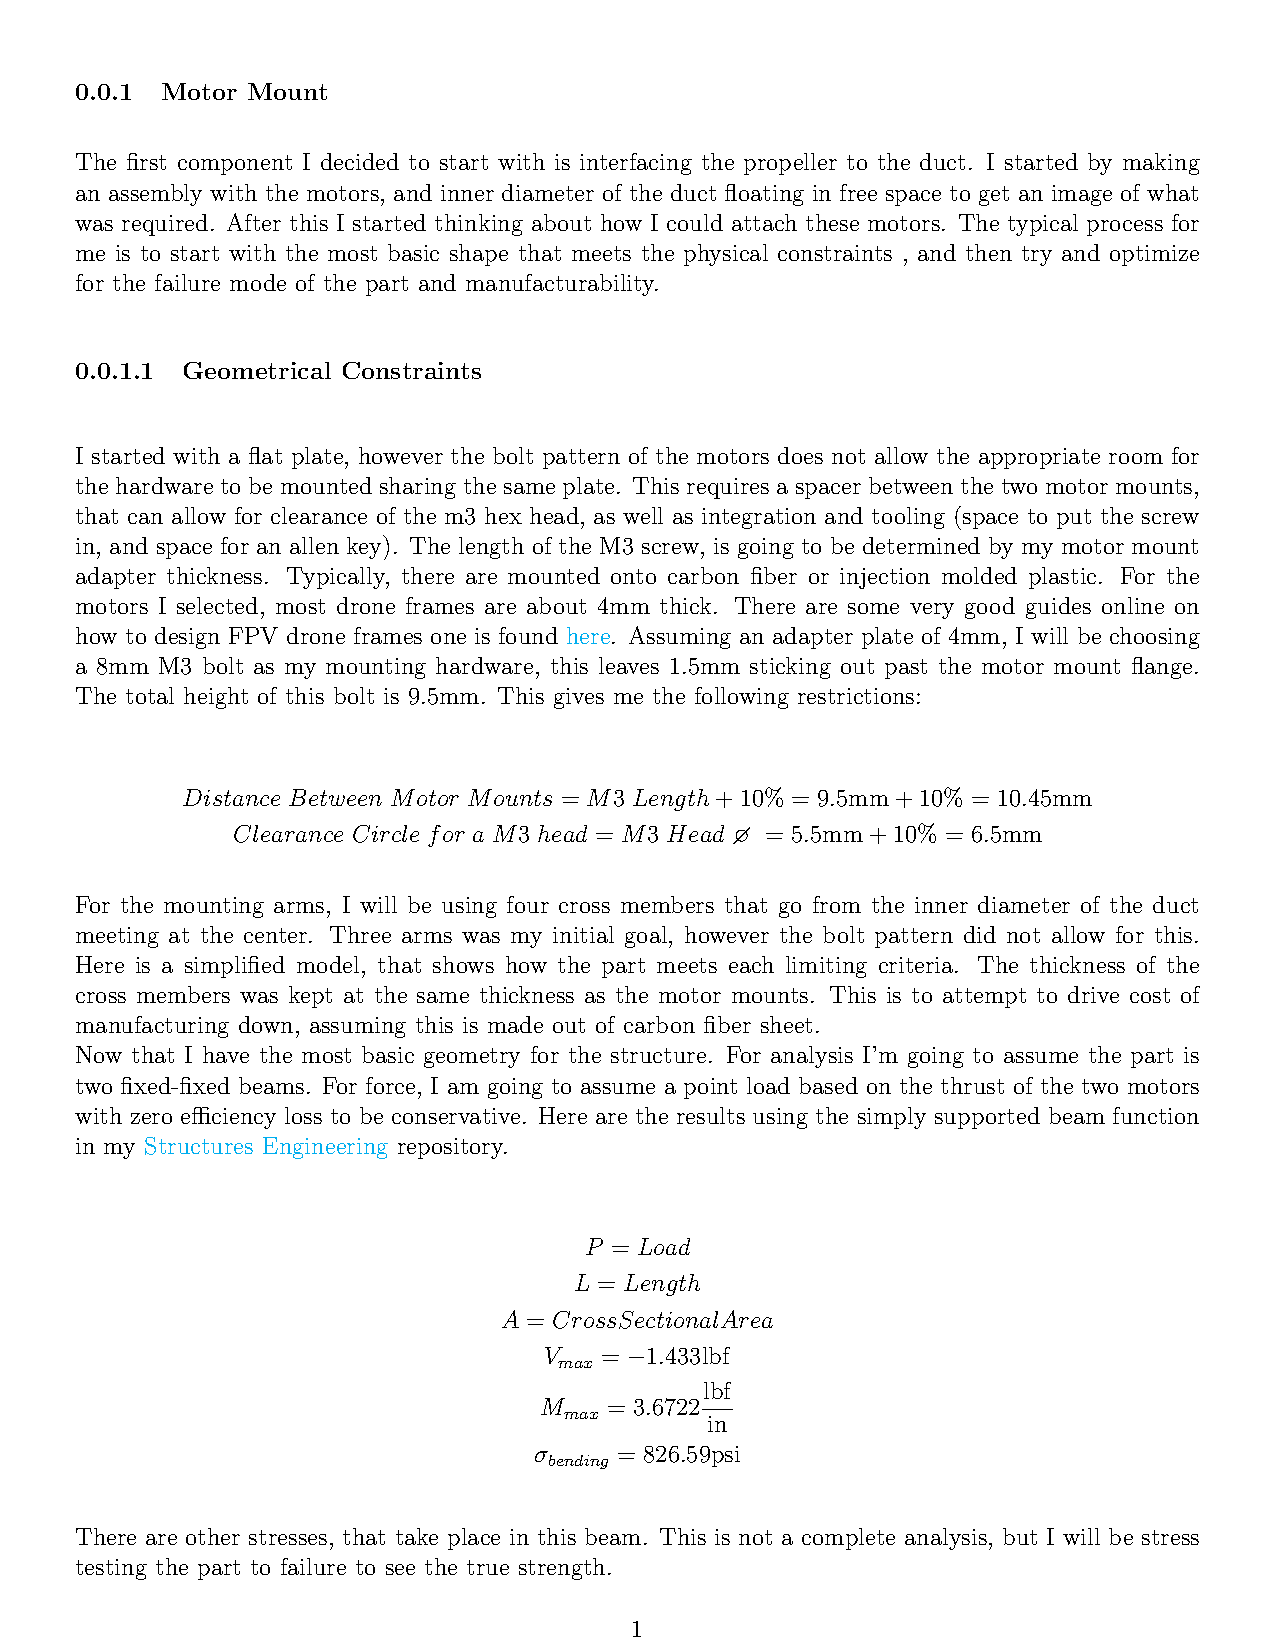
\includegraphics[width = 0.75\textwidth]{Images/Motor Mount/Motor Mount.PNG}
    \caption{}
    \label{fig:my_label}
\end{figure}
\\
Now that I have the most basic geometry for the structure. For analysis I'm going to assume the part is two fixed-fixed beams. For force, I am going to assume a point load based on the thrust of the two motors with zero efficiency loss to be conservative. Here are the results using the simply supported beam function in my \href{https://github.com/ControlSoup/StructuresEngineering}{Structures Engineering} repository.



\begin{figure}[h]
    \centering
    \includegraphics[width = 0.5\textwidth]{Images/simplysupported.png}
    \caption{}
    \label{fig:my_label}
\end{figure}


\begin{gather*}
    P = Load\\
    L= Length\\
    A = Cross Sectional Area
    \\
    V_{max} = -1.433\unit{\lbf}\\
    M_{max} = 3.6722\unit[per-mode = fraction]{\lbf\per\inch}\\
    \sigma_{bending} = 826.59\unit{\psi}\\
\end{gather*}
There are other stresses, that take place in this beam. This is not a complete analysis, but I will be stress testing the part to failure to see the true strength.



\paragraph{Material and Cross Section Optimization}
\setcounter{tocdepth}{4}
\setcounter{secnumdepth}{4}
\mbox{}\\\\
\begin{figure}[h]
    \centering
    \includegraphics[width = 0.75\textwidth]{Images/Buckling Optimizer_v1.png}
    \caption{Motor Mount Optimization Tree}
    \label{fig:my_label}
\end{figure}
For each material I will iterate through the geometrical constraints, looking for a combinations that have a bending FOS greater than two. After that I will double check the deflection is very low, based on intuition, I want this beam to have a maximum deflection of no more than 0.02\unit{\inch}.

\subparagraph{Carbon Fiber}
\mbox{}\\


The material properties for Carbon fiber are notoriously hard to predict with out doing your own testing. This is made considerably harder by the fact that I don't think a carbon fiber sheet on its side has the same material proprieties as a sheet in its nominal direction. This is probably negates my results, but I want to see what the hand calculations expect based on some conservative carbon fiber properties. AGATE CARBON PAPER ETD material properties are as follows:
\begin{gather*}
Density = 1.35\unit[per-mode = fraction]{\g\per\cm\tothe{3}} = 0.0488\unit[per-mode = fraction]{\lb\per\inch\tothe{3}}\\
Ultimate\;Strength = 57.05\unit{\ksi}\\
Elastic Modulus = 6.77\unit{\Msi}
\end{gather*}
The optimization needs to be modified slightly. Carbon fiber sheets come in a select number of thickness, The thickness is what will determine my beam width. The following sizes where available I've included all the common options including 4mm found \href{https://protechcomposites.com/resources/standard-thicknesses}{here}. Additionally because our material properties are not very well known, and I am using the ultimate strength instead of yield, I will be optimizing to a FOS of 3 on the ultimate strength.

The results where as follows:
\begin{gather*}
Cross\;Section\;Width = 0.254\unit{\mm}\\
Cross\;Section\;Height = 10.6\unit{\mm}\\
\sigma_{max} = 1.834\unit{pa}\\
FOS_{buckling} = 4.5\\
Deflection = 0.498\unit{mm}\\
Weight\;of\;Each\;Beam = 0.473\unit{g}
\end{gather*}
\subparagraph{Aluminum}
\mbox{}\\


The properties of aluminum are well know, 7075 T6 has the following properties:
\begin{gather*}
Density = 0.102\unit[per-mode = fraction]{\lb\per\inch\tothe{3}}\\
Yield\;Strength = 83\unit{\ksi}\\
Elastic Modulus = 4.06\unit{\Msi}
\end{gather*}

The optimization will not need modification, a minimum thickness of 0.25\unit{mm} was selected arbitrarily. I need a better model of failure to understand width limits. 

The optimization results where as follows:
\begin{gather*}
Cross\;Section\;Width = 0.25\unit{\mm}\\
Cross\;Section\;Height = 10.45\unit{\mm}\\
\sigma_{max} = 1.918\unit{pa}\\
FOS_{buckling} = 5.52\\
Deflection = 0.344\unit{mm}\\
Weight\;of\;Each\;Beam = 0.96\unit{\g}
\end{gather*}

\subparagraph{3D Printed PLA}
\mbox{}\\

3d printing is a fantastic option for small scale prototyping like I am attempting here. Unfortunately, PLA acts extremely nonlinear under load. Again like carbon fiber, this most likely negates the results of my optimization. However, using some papers that can be found online I can attempt to get an initial guess at the strength of my part for initial design purposes. 

The material properties where pulled from Paper1, and paper2 assuming 70\% infill and are as follows:
\begin{gather*}
Density = 0.0316\unit[per-mode = fraction]{\lb\per\inch\tothe{3}}\\
Yield\;Strength = 2.5\unit{\ksi}\\
Elastic Modulus = 0.123\unit{\Msi}
\end{gather*}

The optimization results where as follows:
\begin{gather*}
Cross\;Section\;Width = 1.06\unit{\mm}\\
Cross\;Section\;Height = 25\unit{\mm}\\
\sigma_{max} = 0.079\unit{pa}\\
FOS_{buckling} = 4.65\\
Deflection = 0.497\unit{mm}\\
Weight\;of\;Each\;Beam = 3.033\unit{\g}
\end{gather*}


\paragraph{Final Selection and Conceptual Design}
\setcounter{tocdepth}{4}
\setcounter{secnumdepth}{4}
\mbox{}\\\\
Based on these three materials, the optimal choice would be a carbon fiber sheet design. My optimization does not take into a account, torsional buckling, misalignment or the torque applied on the part by the motors when not spinning at the same speed. If I had access to some sort of FEA or analysis software I could be more confident in my design. However my confidence would still  not be high due to the uncertainty in the material properties available online. I will need to rely on test results to be sure. Fabrication is a slight concern, I would probably go with several laser/CNC cut sheets that fit together using tabs, and then some kind of epoxy to fixture all of these together. This combination is workable, and could be an interesting choice. However, the cost is going to be higher, and making multiple to test to failure is out of my budget for this vehicle.

Aluminum, is an extremely good choice here, the material properties are extremely well known and the part is really not that heavy. Fabrication would be very difficult, this sheet would be extremely thin. Welding is not an option, some sort of epoxy might work but hardware is probably the best option. 

PLA is going to be my choice, even though its the worst choice. The material properties are less reliable than carbon fiber, and it creates a substantially heavier piece. However, I am going to be relying on strength testing for all of these, due to my optimization being limited. 3d printing allows me to produce a lot of these parts break them, and modify until I am happy with the part. This also opens up the options of eliminating hardware, which at this scale could save enough weight to break even.

\pagebreak
Here is final design, making modifications based on intuition, and rounding optimization results: 
\begin{figure}[h]
    \centering
    \includegraphics[width =0.6\textwidth]{Images/mo/Final_Motor_Mount.PNG}
    \caption{}
    \label{fig:my_label}
\end{figure}

The final hand calcs for failure are:
\begin{gather*}
Cross\;Section\;Width = 1.\unit{\mm}\\
Cross\;Section\;Height = 25\unit{\mm}\\
\sigma_{max} = 0.083\unit{pa}\\
FOS_{buckling} = 4.36\\
Deflection = 0.53\unit{mm}\\
Weight\;of\;Each\;Beam = 2.87\unit{\g}
\end{gather*}

\pagebreak
\paragraph{Testing Results and Changes}
\setcounter{tocdepth}{4}
\setcounter{secnumdepth}{4}
\mbox{}\\\\
\begin{figure}[h]
    \centering
    \includegraphics[width = 0.4\textwidth]{Images/Motor Mount/Motor Mount V1.PNG}
    \caption{Initial Print Mass}
    \label{fig:my_label}
\end{figure}\\
Initial print, gave me the idea to bring the actual mounting main mount down into the beams, this requires a larger minimum height for the column. Is defiantly strong enough, however deflection of off load axis is high. Suggest thickening sides in case of misalignment or torque. Struts are not available due to the space and print-ability. Notes about expected vs actual I ended up having to use 80\% infill material properties have been adjusted also an error in my material properties was found:
\begin{gather*}
\rho = 0.03612\unit{\lb\per\in\tothe{3}}
S_y = 3306.86\unit{\psi}
E = 203052.8\unit{\psi}
\end{gather*}

Force distribution if misalignment of thrust is 5\unit{\degree}
\begin{gather*}
Thrust = 2600\unit{g}\\
F_y = 2600\unit{g} * \cos{5\unit{\degree}} = 226.6\unit{g}\\
F_x = 2600\unit{g} * \sin{5\unit{\degree}} = 2590.1\unit{g}
\end{gather*}
Based on this, one tenth of the expected thrust should be used as a side load (260\unit{g}).

Deflection is my primary concern, however because the side load is in reality supported by another beam perpendicular to the one I am analyzing, I am willing to allow three times as much deflection (1.5\unit{mm}) I will need to see in testing if this will work out.
\pagebreak
\begin{figure}[h]
    \centering
    \includegraphics[width = 1\textwidth]{Images/Motor Mount Optimization_V2png.png}
    \caption{Motor Mount Optimization Tree V2}
    \label{fig:my_label}
\end{figure}\\

Results of this optimization are:

\begin{gather*}
Cross\;Section\;Width = 2.638\unit{\mm}\\
Cross\;Section\;Height = 18.45\unit{\mm}\\
FOS_{vertical} = 8.223\\
FOS_{horizontal} = 11.756\\
Deflection_{vertical} = 0.303\unit{mm}\\
Deflection_{horizontal} = 1.382\\
Weight\;of\;Each\;Beam = 6.335\unit{\g}
\end{gather*}

New Part Model:
\begin{figure}[h]
    \centering
    \includegraphics[width = 0.5\textwidth]{Images/Motor Mount/Motor Mount V2.PNG}
    \caption{}
    \label{fig:my_label}
\end{figure}\\

\subparagraph{Test Results}



\end{document}